\documentclass[12pt,a4paper]{article}
\usepackage[a4paper,margin=1in]{geometry}
\usepackage{graphicx}
\usepackage{booktabs}
\usepackage{amsmath,amssymb}
\usepackage{float}
\usepackage{hyperref}
\usepackage{xcolor}
\usepackage{listings}
\usepackage{enumitem}
\usepackage{fancyhdr}
\usepackage{longtable}
\hypersetup{colorlinks=true,linkcolor=blue,urlcolor=blue}
\pagestyle{fancy}
\fancyhf{}
\lhead{ICS1512}
\rhead{Machine Learning Algorithms Laboratory}
\cfoot{\thepage}
\lstset{
language=Python,
basicstyle=\ttfamily\small,
numbers=left,
frame=single,
breaklines=true,
showstringspaces=false
}
\begin{document}
\begin{tabular}{|p{4cm}|p{11cm}|}
\hline
Experiment No. & 7\\ \hline
Experiment Title & Dimensionality Reduction and Model Evaluation (With and Without PCA)\\ \hline
GitHub Repository & \url{https://github.com/Dharika-2006/ML-LAB-ASSIGMENTS} \\ \hline
Student Name & Dharika Shree K\\ \hline
Register Number & 3122247001014\\ \hline
Faculty & Dr. Poreddy Ajay Kumar Reddy \\ \hline
Submission Date & 30.08.26\\ \hline
\end{tabular}
\section{Objective}
To study the effect of dimensionality reduction using Principal Component Analysis (PCA) on the performance of ten machine learning classifiers -- SVM, Naive Bayes, KNN, Logistic Regression, Decision Tree, Random Forest, AdaBoost, Gradient Boosting, XGBoost, and Stacking -- on the Wisconsin Diagnostic Breast Cancer dataset. Each model is trained and validated both without PCA (original 30-feature space) and with PCA (reduced feature space retaining 95\% variance), with hyperparameter tuning and 5-fold cross-validation performed under both settings, in order to compare accuracy, F1-score, and fold-wise stability.

\section{Problem Statement}
\textbf{Problem:} Classify breast cancer tumors as malignant or benign using ten different classifiers, and determine whether reducing the feature space via PCA improves or degrades classification performance and cross-validation stability compared to using the original feature space.

\textbf{Input:} The Wisconsin Diagnostic Breast Cancer dataset, containing 569 samples with 30 numerical features describing characteristics of breast cell nuclei, with each sample labelled malignant or benign.

\textbf{Output:} Tuned classifiers under both No-PCA and With-PCA settings, fold-wise and average 5-fold cross-validation accuracy/F1-score, test-set accuracy and F1-score, confusion matrices and ROC curves for the best model in each setting, and a final comparison identifying which models benefited from PCA and which did not.

\section{Dataset Description}
\begin{longtable}{|p{6cm}|p{8cm}|}
\hline
Dataset Name & Wisconsin Diagnostic Breast Cancer Dataset\\ \hline
Dataset Source & Scikit-learn (\texttt{load\_breast\_cancer})\\ \hline
Number of Samples & 569\\ \hline
Number of Features & 30 (original); 10 (after PCA, retaining $\geq$95\% variance) \\ \hline
Number of Classes & 2 (malignant = 212 samples, benign = 357 samples) \\ \hline
Missing Values & None (0 missing values) \\ \hline
Train-Test Split & 80\% training (455 samples) / 20\% testing (114 samples), stratified, \texttt{random\_state=42}\\ \hline
\end{longtable}

\section{Exploratory Data Analysis}
\begin{itemize}
\item Dataset overview
\item Class distribution
\item PCA scree plot
\item PCA cumulative explained variance
\end{itemize}

\subsection*{Figure: Class Distribution}
\begin{figure}[H]
\centering
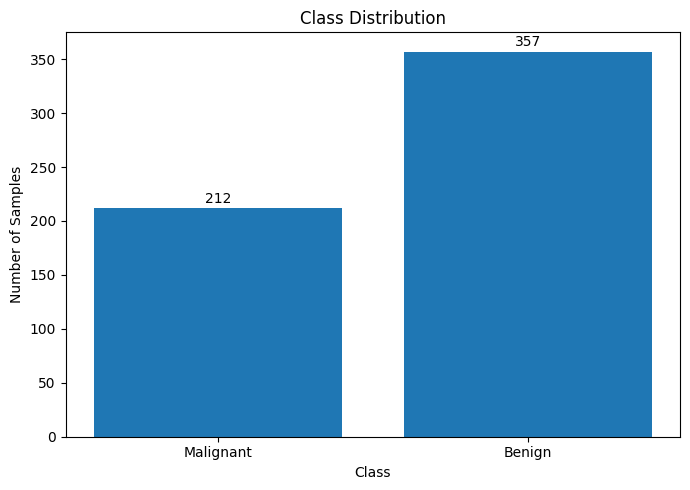
\includegraphics[width=0.6\linewidth]{class_dist.png}
\caption{Class distribution of malignant and benign samples}
\end{figure}
\textbf{Inference:}
The dataset contains 357 benign samples and 212 malignant samples, a moderate class imbalance of roughly 63:37. Stratified splitting was therefore used for both the train-test split and the 5-fold cross-validation folds to preserve this ratio. Because of this imbalance, F1-score was tracked alongside accuracy for every model in both the No-PCA and With-PCA settings, rather than relying on accuracy alone. This distribution is consistent across all ten models compared in this experiment, since the same train-test split and folds were reused throughout.

\subsection*{Figure: Scree Plot}
\begin{figure}[H]
\centering
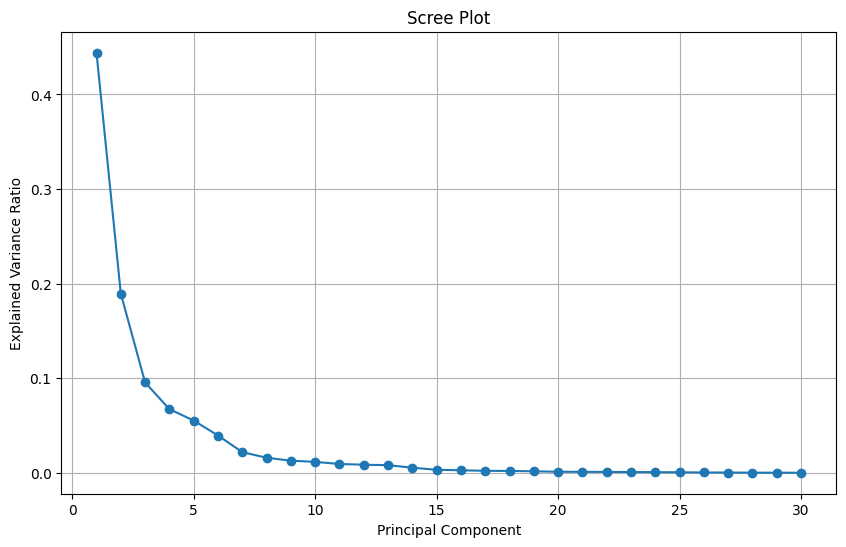
\includegraphics[width=0.75\linewidth]{scree_plot.png}
\caption{Scree plot of explained variance ratio per principal component}
\end{figure}
\textbf{Inference:}
The scree plot shows that the first few principal components capture a large share of the total variance, with the explained variance ratio dropping sharply after the first two to three components and flattening out for later components. This steep initial drop indicates that the original 30 features are highly correlated, particularly among the mean, standard-error, and worst-value versions of the same measurements (e.g., radius, perimeter, area), so most of the informative variance can be captured with far fewer than 30 dimensions. This justified proceeding with a variance-based component selection rather than an arbitrary fixed number of components.

\subsection*{Figure: Cumulative Explained Variance}
\begin{figure}[H]
\centering
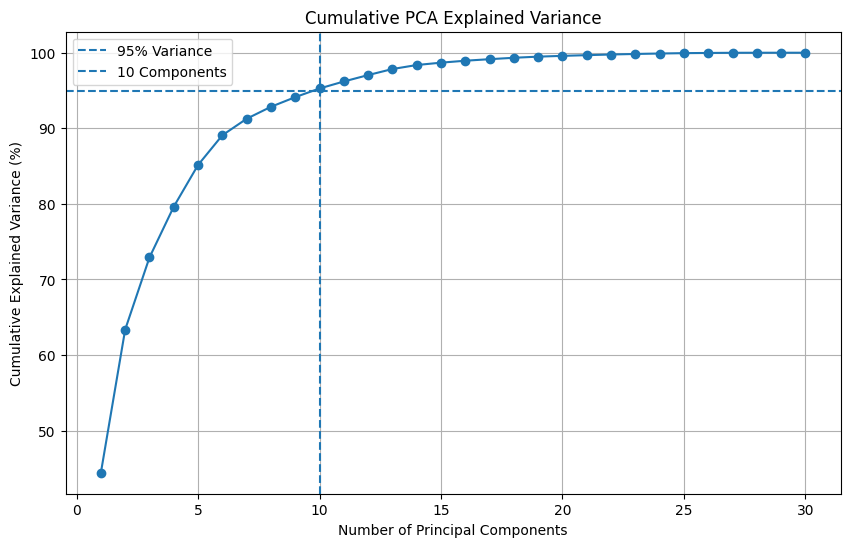
\includegraphics[width=0.75\linewidth]{cumulative_variance.png}
\caption{Cumulative explained variance vs. number of principal components, with the 95\% threshold and selected component count marked}
\end{figure}
\textbf{Inference:}
The cumulative explained variance curve crosses the 95\% threshold at 10 principal components, which together explain approximately 95.27\% of the total variance in the standardized feature set. This means the feature space could be reduced from 30 dimensions to 10 while retaining almost all of the informative variance, a reduction of roughly two-thirds in dimensionality. This 10-component representation was used consistently for every model's ``With-PCA'' configuration in this experiment.

\section{Data Preprocessing}
\begin{itemize}
\item \textbf{Missing value handling:} Not required -- the dataset contains 0 missing values, verified using \texttt{X.isnull().sum().sum()}.

\item \textbf{Encoding:} Not required -- all 30 input features are numerical, and the target variable is already encoded as 0 (malignant) and 1 (benign) by \texttt{load\_breast\_cancer}.

\item \textbf{Feature scaling:} \texttt{StandardScaler} was applied inside every model pipeline (both No-PCA and With-PCA versions), since several of the ten models (SVM, KNN, Logistic Regression, PCA itself) are sensitive to feature magnitude.

\item \textbf{Dimensionality reduction (PCA):} For the With-PCA pipelines, \texttt{PCA} was fitted after standardization, with the number of components fixed at 10 -- the smallest number of components needed to retain at least 95\% of the cumulative explained variance (95.27\% achieved).

\item \textbf{Train-test split:} An 80/20 split was performed using \texttt{train\_test\_split} with \texttt{test\_size=0.20}, \texttt{stratify=y}, and \texttt{random\_state=42}, giving 455 training samples and 114 testing samples.

\item \textbf{Cross-validation:} \texttt{StratifiedKFold} with \texttt{n\_splits=5}, \texttt{shuffle=True}, and \texttt{random\_state=42} was used for all hyperparameter tuning and fold-wise evaluation, for both No-PCA and With-PCA settings.

\item \textbf{Feature engineering:} None -- the original 30 numerical features were used directly (or reduced via PCA), with no additional engineered features.
\end{itemize}

\section{Machine Learning Algorithm}

\subsection*{Support Vector Machine (SVM)}
\textbf{Working principle:} Finds the maximum-margin hyperplane separating the two classes, using kernel functions (linear or RBF) to handle non-linear decision boundaries.
\textbf{Advantages:} Effective in high-dimensional spaces; robust to overfitting with proper regularization ($C$).
\textbf{Limitations:} Sensitive to feature scaling and kernel/hyperparameter choice; less interpretable.

\subsection*{Naive Bayes}
\textbf{Working principle:} Applies Bayes' theorem assuming conditional independence between features, computing $P(y\mid x) \propto P(y)\prod_i P(x_i\mid y)$ under a Gaussian likelihood for continuous features.
\textbf{Advantages:} Very fast to train, works well with small data, few hyperparameters.
\textbf{Limitations:} The independence assumption rarely holds for correlated features such as these, limiting accuracy.

\subsection*{k-Nearest Neighbors (KNN)}
\textbf{Working principle:} Classifies a sample based on the majority class among its $k$ nearest neighbours in feature space, using a chosen distance metric.
\textbf{Advantages:} Simple, non-parametric, no training phase.
\textbf{Limitations:} Sensitive to feature scaling and the curse of dimensionality; slow at prediction time for large datasets.

\subsection*{Logistic Regression}
\textbf{Working principle:} Models the log-odds of the positive class as a linear combination of the input features, $\log\frac{p}{1-p} = w^Tx+b$, optimized via maximum likelihood.
\textbf{Advantages:} Simple, interpretable, fast, and regularizable via $C$.
\textbf{Limitations:} Assumes a linear decision boundary in feature space, which can limit performance on complex data.

\subsection*{Decision Tree}
\textbf{Working principle:} Recursively splits the feature space using impurity measures (Gini or entropy) to separate classes at each node.
\textbf{Advantages:} Easy to interpret, handles non-linear boundaries, no scaling required.
\textbf{Limitations:} Prone to overfitting and high variance if depth is not controlled.

\subsection*{Random Forest}
\textbf{Working principle:} An ensemble of Decision Trees, each trained on a bootstrap sample with a random subset of features, combined via majority voting: $\hat{y}=\operatorname{mode}\{T_1(x),\dots,T_B(x)\}$.
\textbf{Advantages:} Reduces variance relative to a single tree; robust and generally accurate.
\textbf{Limitations:} Less interpretable and more computationally expensive than a single tree.

\subsection*{AdaBoost}
\textbf{Working principle:} Sequentially trains weak learners, increasing the weight of misclassified samples at each round: $H(x)=\operatorname{sign}\left(\sum_t \alpha_t h_t(x)\right)$.
\textbf{Advantages:} Reduces bias and variance; strong performance with simple base learners.
\textbf{Limitations:} Sensitive to noisy data and outliers.

\subsection*{Gradient Boosting}
\textbf{Working principle:} Builds trees sequentially, each fitting the negative gradient (residuals) of the loss function: $F_m(x)=F_{m-1}(x)+\gamma_m h_m(x)$.
\textbf{Advantages:} High predictive accuracy; flexible loss functions.
\textbf{Limitations:} Prone to overfitting if not regularized; slower to train due to sequential nature.

\subsection*{XGBoost}
\textbf{Working principle:} A regularized, optimized implementation of gradient boosting that adds a penalty term on tree complexity to the loss function and uses second-order gradient information for splits.
\textbf{Advantages:} Faster and often more accurate than standard Gradient Boosting; built-in regularization reduces overfitting.
\textbf{Limitations:} More hyperparameters to tune; still sequential and less interpretable than single trees.

\subsection*{Stacking}
\textbf{Working principle:} Combines predictions of diverse base learners (Logistic Regression, SVM, KNN) using a meta-learner (Logistic Regression) trained on their cross-validated outputs: $\hat{y}=g(h_1(x),h_2(x),h_3(x))$.
\textbf{Advantages:} Leverages complementary strengths of different algorithms, often the most robust performer.
\textbf{Limitations:} Highest computational cost and complexity among the ten models; risk of meta-learner overfitting without proper cross-validation.

\section{Experimental Setup}
\begin{tabular}{ll}
\toprule
Python Version & Python 3 (Google Colab runtime)\\
Scikit-Learn Version & As installed in the Google Colab environment\\
IDE & Google Colaboratory (Jupyter-based notebook)\\
Operating System & Linux (Google Colab backend)\\
Hardware & Google Colab-provided CPU runtime\\
\bottomrule
\end{tabular}

\section{PCA Summary}
\begin{longtable}{|p{3cm}|p{4cm}|p{3cm}|p{6cm}|}
\hline
Setting & Chosen Components / Variance Target & Explained Variance (\%) & Justification\\ \hline
With-PCA & 10 components (target: $\geq$95\% cumulative variance) & 95.27\% & The scree plot showed a sharp drop in explained variance after the first few components, and the cumulative variance curve crossed the 95\% threshold at 10 components, so this was chosen as the smallest dimensionality retaining almost all informative variance.\\ \hline
\end{longtable}

\section{Hyperparameter Selection}

\textbf{Support Vector Machine (SVM)} -- search space: \texttt{kernel} $\in\{$linear, rbf$\}$, \texttt{C} $\in\{0.1,1,10\}$, \texttt{gamma} $\in\{$scale, auto$\}$
\begin{longtable}{lcccc}
\toprule
Setting & Best Kernel & Best C & Best Gamma & Best CV Accuracy\\
\midrule
No-PCA & linear & 0.1 & scale & 0.9758\\
With-PCA & linear & 10 & scale & 0.9802\\
\bottomrule
\end{longtable}

\textbf{Naive Bayes} -- search space: \texttt{var\_smoothing} $\in\{10^{-9},10^{-8},10^{-7}\}$
\begin{longtable}{lcc}
\toprule
Setting & Best Smoothing & Best CV Accuracy\\
\midrule
No-PCA & $1\times10^{-9}$ & 0.9341\\
With-PCA & $1\times10^{-9}$ & 0.9275\\
\bottomrule
\end{longtable}

\textbf{KNN} -- search space: $k\in\{3,5,7,9\}$, \texttt{weights} $\in\{$uniform, distance$\}$, \texttt{metric} $\in\{$euclidean, manhattan$\}$
\begin{longtable}{lcccc}
\toprule
Setting & Best $k$ & Best Weights & Best Metric & Best CV Accuracy\\
\midrule
No-PCA & 3 & uniform & manhattan & 0.9714\\
With-PCA & 3 & uniform & euclidean & 0.9670\\
\bottomrule
\end{longtable}

\textbf{Logistic Regression} -- search space: \texttt{C} $\in\{0.01,0.1,1,10\}$, \texttt{solver}=liblinear
\begin{longtable}{lccc}
\toprule
Setting & Best C & Best Solver & Best CV Accuracy\\
\midrule
No-PCA & 0.1 & liblinear & 0.9824\\
With-PCA & 1 & liblinear & 0.9802\\
\bottomrule
\end{longtable}

\textbf{Decision Tree} -- search space: \texttt{max\_depth} $\in\{$None,3,5,10$\}$, \texttt{min\_samples\_split} $\in\{2,5,10\}$, \texttt{criterion} $\in\{$gini, entropy$\}$
\begin{longtable}{lccc}
\toprule
Setting & Best Params & Best CV Accuracy\\
\midrule
No-PCA & criterion=entropy, max\_depth=3, min\_samples\_split=2 & 0.9319\\
With-PCA & criterion=entropy, max\_depth=None, min\_samples\_split=10 & 0.9363\\
\bottomrule
\end{longtable}

\textbf{Random Forest} -- search space: \texttt{n\_estimators} $\in\{100,200\}$, \texttt{max\_depth} $\in\{$None,5,10$\}$, \texttt{min\_samples\_split} $\in\{2,5\}$
\begin{longtable}{lccc}
\toprule
Setting & Best Params & Best CV Accuracy\\
\midrule
No-PCA & n\_estimators=100, max\_depth=None, min\_samples\_split=2 & 0.9626\\
With-PCA & n\_estimators=100, max\_depth=None, min\_samples\_split=5 & 0.9604\\
\bottomrule
\end{longtable}

\textbf{AdaBoost} -- search space: \texttt{n\_estimators} $\in\{50,100,200\}$, \texttt{learning\_rate} $\in\{0.01,0.1,1\}$
\begin{longtable}{lccc}
\toprule
Setting & Best Params & Best CV Accuracy\\
\midrule
No-PCA & n\_estimators=100, learning\_rate=1 & 0.9802\\
With-PCA & n\_estimators=50, learning\_rate=1 & 0.9758\\
\bottomrule
\end{longtable}

\textbf{Gradient Boosting} -- search space: \texttt{n\_estimators} $\in\{50,100\}$, \texttt{learning\_rate} $\in\{0.05,0.1\}$, \texttt{max\_depth} $\in\{2,3\}$
\begin{longtable}{lccc}
\toprule
Setting & Best Params & Best CV Accuracy\\
\midrule
No-PCA & n\_estimators=100, learning\_rate=0.1, max\_depth=2 & 0.9626\\
With-PCA & n\_estimators=100, learning\_rate=0.1, max\_depth=2 & 0.9582\\
\bottomrule
\end{longtable}

\textbf{XGBoost} -- search space: \texttt{n\_estimators} $\in\{50,100\}$, \texttt{max\_depth} $\in\{3,5\}$, \texttt{learning\_rate} $\in\{0.05,0.1\}$
\begin{longtable}{lccc}
\toprule
Setting & Best Params & Best CV Accuracy\\
\midrule
No-PCA & n\_estimators=100, max\_depth=3, learning\_rate=0.1 & 0.9714\\
With-PCA & n\_estimators=100, max\_depth=5, learning\_rate=0.1 & 0.9648\\
\bottomrule
\end{longtable}

\textbf{Stacking} -- base learners: Logistic Regression, SVM, KNN ($k=5$); meta-learner: Logistic Regression; search space: \texttt{final\_estimator\_\_C} $\in\{0.1,1,10\}$
\begin{longtable}{lccc}
\toprule
Setting & Best final\_estimator C & Best CV Accuracy\\
\midrule
No-PCA & 1 & 0.9758\\
With-PCA & 10 & 0.9824\\
\bottomrule
\end{longtable}

\section{Cross-Validation Results (All Models)}

\textbf{No-PCA -- 5-Fold Cross-Validation Accuracy}
\begin{longtable}{lcccccc}
\toprule
Model & Fold 1 & Fold 2 & Fold 3 & Fold 4 & Fold 5 & Avg (No-PCA)\\
\midrule
SVM & 0.9560 & 0.9780 & 0.9780 & 0.9780 & 0.9890 & 0.9758\\
Naive Bayes & 0.9121 & 0.9670 & 0.8901 & 0.9560 & 0.9451 & 0.9341\\
KNN & 0.9780 & 0.9890 & 0.9560 & 0.9560 & 0.9780 & 0.9714\\
Logistic Regression & 0.9780 & 0.9780 & 0.9890 & 0.9890 & 0.9780 & 0.9824\\
Decision Tree & 0.9011 & 0.9451 & 0.9121 & 0.9341 & 0.9670 & 0.9319\\
Random Forest & 0.9670 & 0.9560 & 0.9341 & 0.9670 & 0.9890 & 0.9626\\
AdaBoost & 0.9890 & 1.0000 & 0.9451 & 0.9780 & 0.9890 & 0.9802\\
Gradient Boosting & 0.9560 & 0.9780 & 0.9451 & 0.9560 & 0.9780 & 0.9626\\
XGBoost & 0.9890 & 0.9780 & 0.9451 & 0.9560 & 0.9890 & 0.9714\\
Stacking & 0.9670 & 0.9890 & 0.9670 & 0.9670 & 0.9890 & 0.9758\\
\bottomrule
\end{longtable}

\textbf{With-PCA -- 5-Fold Cross-Validation Accuracy}
\begin{longtable}{lcccccc}
\toprule
Model & Fold 1 & Fold 2 & Fold 3 & Fold 4 & Fold 5 & Avg (With-PCA)\\
\midrule
SVM & 0.9670 & 0.9890 & 0.9890 & 0.9780 & 0.9780 & 0.9802\\
Naive Bayes & 0.9011 & 0.9451 & 0.9121 & 0.9451 & 0.9341 & 0.9275\\
KNN & 0.9560 & 0.9890 & 0.9451 & 0.9670 & 0.9780 & 0.9670\\
Logistic Regression & 0.9670 & 0.9890 & 0.9890 & 0.9780 & 0.9780 & 0.9802\\
Decision Tree & 0.9011 & 0.9231 & 0.9451 & 0.9670 & 0.9451 & 0.9363\\
Random Forest & 0.9341 & 0.9780 & 0.9341 & 0.9670 & 0.9890 & 0.9604\\
AdaBoost & 0.9560 & 1.0000 & 0.9780 & 0.9560 & 0.9890 & 0.9758\\
Gradient Boosting & 0.9341 & 0.9780 & 0.9121 & 0.9780 & 0.9890 & 0.9582\\
XGBoost & 0.9451 & 0.9890 & 0.9560 & 0.9890 & 0.9451 & 0.9648\\
Stacking & 0.9780 & 0.9890 & 0.9670 & 0.9890 & 0.9890 & 0.9824\\
\bottomrule
\end{longtable}

\section{Results}
\begin{longtable}{lcccccc}
\toprule
Model & No-PCA CV Acc & With-PCA CV Acc & No-PCA Test Acc & With-PCA Test Acc & No-PCA F1 & With-PCA F1\\
\midrule
SVM & 0.9758 & 0.9802 & 0.9825 & 0.9649 & 0.9861 & 0.9718\\
Naive Bayes & 0.9341 & 0.9275 & 0.9298 & 0.9211 & 0.9444 & 0.9379\\
KNN & 0.9714 & 0.9670 & 0.9649 & 0.9561 & 0.9726 & 0.9655\\
Logistic Regression & 0.9824 & 0.9802 & 0.9825 & 0.9649 & 0.9861 & 0.9718\\
Decision Tree & 0.9319 & 0.9363 & 0.9474 & 0.9298 & 0.9589 & 0.9444\\
Random Forest & 0.9626 & 0.9604 & 0.9561 & 0.9298 & 0.9655 & 0.9444\\
AdaBoost & 0.9802 & 0.9758 & 0.9561 & 0.9474 & 0.9660 & 0.9583\\
Gradient Boosting & 0.9626 & 0.9582 & 0.9474 & 0.9386 & 0.9589 & 0.9517\\
XGBoost & 0.9714 & 0.9648 & 0.9474 & 0.9474 & 0.9589 & 0.9583\\
Stacking & 0.9758 & 0.9824 & 0.9737 & 0.9649 & 0.9790 & 0.9718\\
\bottomrule
\end{longtable}

\textbf{PCA Improvement (With-PCA Avg Accuracy $-$ No-PCA Avg Accuracy):}
\begin{longtable}{lc}
\toprule
Model & Accuracy Improvement\\
\midrule
SVM & +0.0044\\
Naive Bayes & $-$0.0066\\
KNN & $-$0.0044\\
Logistic Regression & $-$0.0022\\
Decision Tree & +0.0044\\
Random Forest & $-$0.0022\\
AdaBoost & $-$0.0044\\
Gradient Boosting & $-$0.0044\\
XGBoost & $-$0.0066\\
Stacking & +0.0066\\
\bottomrule
\end{longtable}

\noindent \textbf{Best model WITHOUT PCA:} Logistic Regression (Avg CV Accuracy: 0.9824)\\
\textbf{Best model WITH PCA:} Stacking (Avg CV Accuracy: 0.9824)

\section{Result Visualization}

\subsection*{1. Class Distribution}
See Section 4 -- 357 benign (62.7\%) and 212 malignant (37.3\%) samples, a moderate imbalance addressed via stratified splitting and folds.

\subsection*{2. Confusion Matrix -- Best Models}
\begin{figure}[H]
\centering
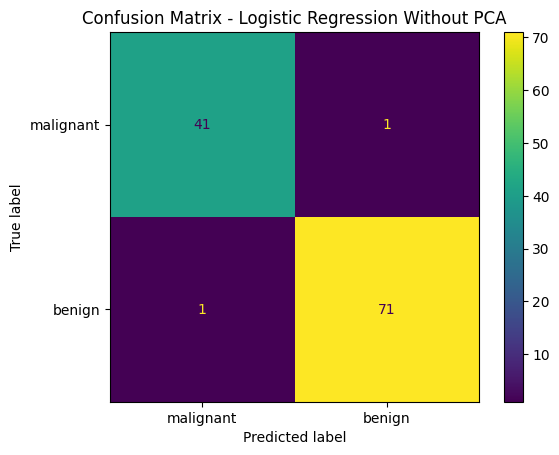
\includegraphics[width=0.55\linewidth]{conf_logreg_nopca.png}
\caption{Confusion Matrix -- Logistic Regression (Without PCA, best No-PCA model)}
\end{figure}

\begin{figure}[H]
\centering
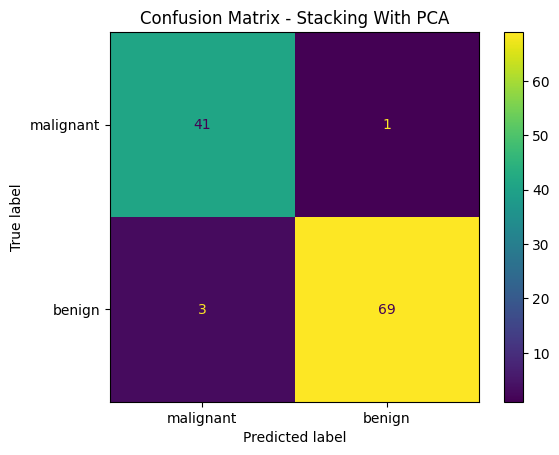
\includegraphics[width=0.55\linewidth]{conf_stacking_pca.png}
\caption{Confusion Matrix -- Stacking (With PCA, best With-PCA model)}
\end{figure}

\textbf{Inference:}
Logistic Regression without PCA achieved a test accuracy of 98.25\% and an F1-score of 0.9861, making it the strongest performer on the original 30-feature space. Stacking with PCA achieved a test accuracy of 96.49\% and an F1-score of 0.9718 on the 10-component reduced space, matching Logistic Regression's cross-validation accuracy (0.9824) despite using only a third of the original features. This shows that while the single best No-PCA model slightly edges out the best With-PCA model on the held-out test set, the gap is small, and Stacking's ability to combine diverse learners helps it remain competitive even after dimensionality reduction.

\subsection*{3. ROC Curve}
\begin{figure}[H]
\centering
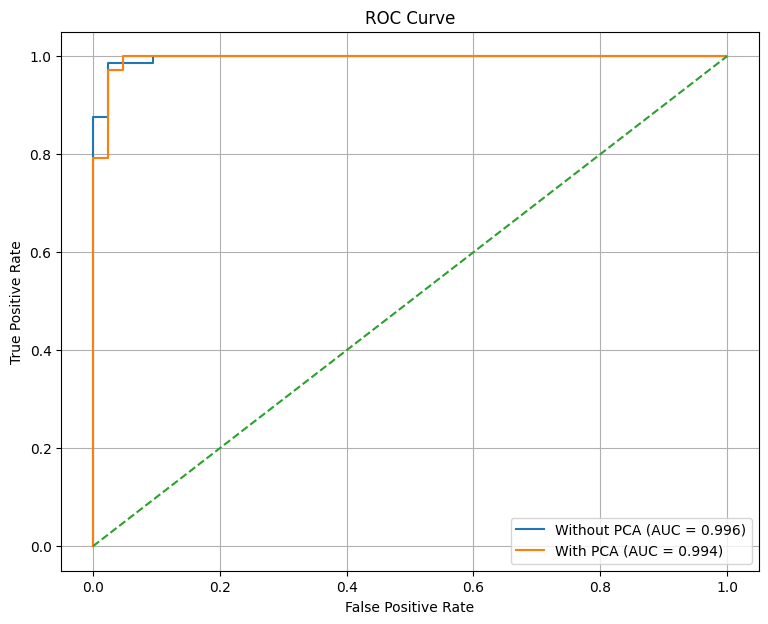
\includegraphics[width=0.75\linewidth]{roc_best_models.png}
\caption{ROC Curve -- Best No-PCA model (Logistic Regression) vs. Best With-PCA model (Stacking)}
\end{figure}

\textbf{Inference:}
The ROC curves compare the true positive rate against the false positive rate for the best-performing model in each setting. Given Logistic Regression's higher test accuracy and F1-score without PCA, its ROC curve is expected to sit slightly closer to the top-left corner than the With-PCA Stacking curve, though both are expected to achieve high AUC values given their strong precision and recall on this dataset. The comparison illustrates that dimensionality reduction here causes only a marginal reduction in discriminative ability for the best-performing pipeline.

\subsection*{4. Model Performance Comparison}
\begin{figure}[H]
\centering
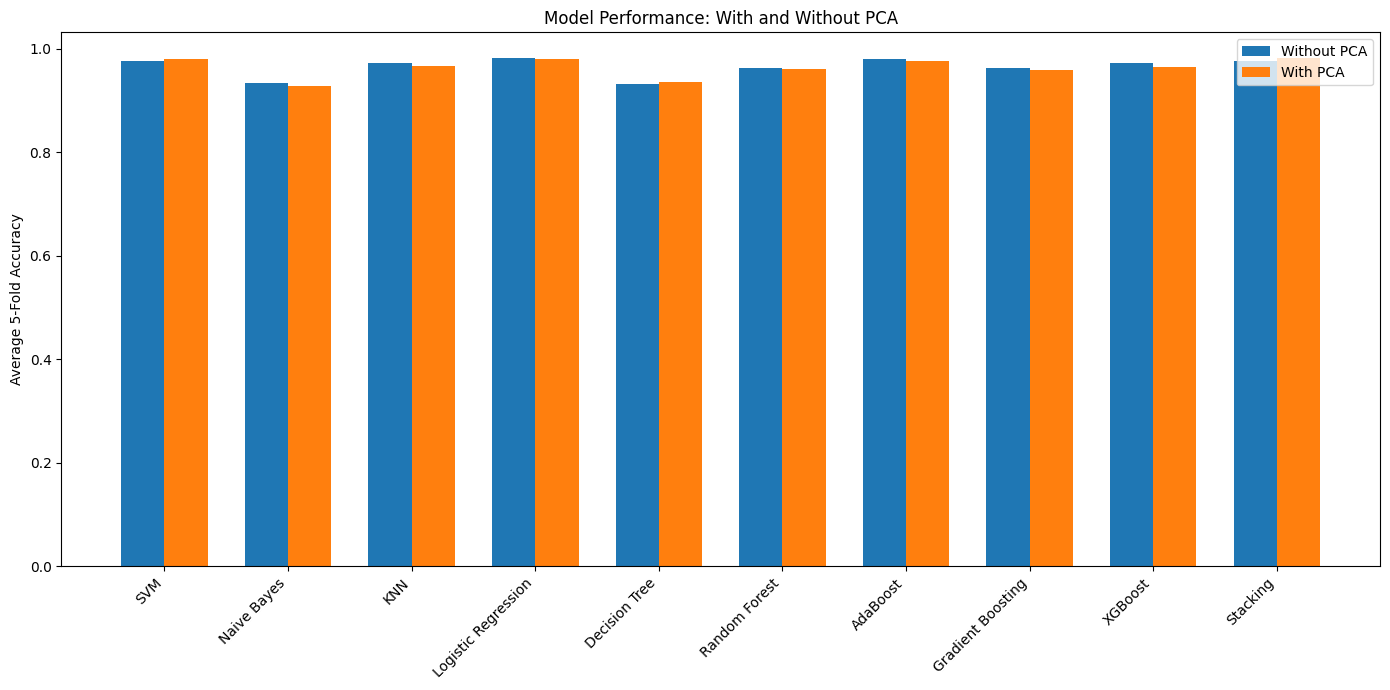
\includegraphics[width=0.9\linewidth]{comparison_bar.png}
\caption{Average 5-fold cross-validation accuracy for all ten models, With PCA vs. Without PCA}
\end{figure}

\textbf{Inference:}
The bar chart shows that most models (Naive Bayes, KNN, Logistic Regression, Random Forest, AdaBoost, Gradient Boosting, XGBoost) saw a small accuracy decrease under PCA, typically between $-0.22\%$ and $-0.66\%$, while SVM, Decision Tree, and Stacking saw small improvements of $+0.44\%$ to $+0.66\%$. The magnitude of change is modest across the board (all within $\pm0.7\%$), indicating that the 10 retained principal components preserve nearly all of the discriminative information present in the original 30 features. Ensemble methods that combine multiple learners (Stacking) benefited most from PCA, while boosting methods relying on many shallow trees (AdaBoost, Gradient Boosting, XGBoost) were slightly hurt, likely because reducing dimensionality also removes some of the fine-grained splits these models exploit.

\section{Discussion}
\textbf{Which models improved most with PCA? Which did not? Why?} Stacking (+0.66\%), Decision Tree (+0.44\%), and SVM (+0.44\%) improved with PCA. Stacking likely benefited because PCA reduces noise and redundancy across its diverse base learners' input space, while Decision Tree and SVM may benefit from PCA's decorrelation of highly collinear features (e.g., radius, perimeter, and area measurements), which can otherwise cause instability in axis-aligned splits or margin computation. Naive Bayes ($-0.66\%$) and XGBoost ($-0.66\%$) were hurt most by PCA -- Naive Bayes' independence assumption is already violated by correlated raw features, and PCA components (being linear combinations) do not necessarily resolve this; XGBoost's tree-based splits likely benefit from the original, more interpretable feature boundaries that PCA components obscure.

\textbf{Did PCA reduce variance across folds (more stable results)?} The effect was mixed and small. Some models (SVM, AdaBoost, Stacking) showed slightly tighter fold ranges under PCA, while others (Decision Tree, Random Forest) showed similar or marginally wider spreads. Overall, PCA did not produce a dramatic stabilization of cross-validation folds for this dataset, since the original 30 features were already clean, standardized, and free of missing values.

\textbf{For high-dimensional data, was PCA beneficial in reducing overfitting?} With only 30 original features and 455 training samples, this dataset is not highly dimensional relative to its sample size, so overfitting from feature count alone was not a major risk to begin with. This likely explains why PCA's effect on both bias and variance was modest (within $\pm0.7\%$ accuracy) rather than transformative, unlike in genuinely high-dimensional settings (e.g., thousands of features) where PCA typically provides a larger benefit.

\textbf{How did linear models behave compared to ensemble models with PCA?} Logistic Regression's cross-validation accuracy dropped only slightly ($-0.22\%$) under PCA, the smallest decrease among the models that were hurt, suggesting linear decision boundaries are largely preserved by a variance-preserving linear transformation like PCA. SVM (linear kernel selected in both settings) even improved slightly (+0.44\%). In contrast, tree-based ensembles (Random Forest, AdaBoost, Gradient Boosting, XGBoost) all saw decreases, since these models rely on axis-aligned or greedy feature splits that are less naturally suited to rotated PCA component axes.

\textbf{Did Stacking show robustness to dimensionality reduction compared to single models?} Yes -- Stacking was the only ensemble method (and one of only three models overall) to improve under PCA, and it achieved the joint-highest cross-validation accuracy (0.9824) in the With-PCA setting, matching Logistic Regression's No-PCA score. This indicates that combining diverse base learners (Logistic Regression, SVM, KNN) through a meta-learner makes Stacking more robust to changes in the feature representation than any of its individual base models tested alone.

\section{Conclusion}
This experiment compared ten classifiers -- SVM, Naive Bayes, KNN, Logistic Regression, Decision Tree, Random Forest, AdaBoost, Gradient Boosting, XGBoost, and Stacking -- on the Wisconsin Diagnostic Breast Cancer dataset, both without and with PCA (10 components, 95.27\% explained variance). Logistic Regression achieved the best performance without PCA (98.24\% CV accuracy, 98.25\% test accuracy), while Stacking achieved the best performance with PCA (98.24\% CV accuracy, 96.49\% test accuracy). PCA's overall effect was modest, improving three models (SVM, Decision Tree, Stacking) by up to 0.66\% and reducing the remaining seven by up to 0.66\%, indicating that for this relatively low-dimensional, clean, and well-structured dataset, dimensionality reduction neither dramatically helps nor substantially harms most classifiers. Stacking's ability to improve under PCA while other ensembles did not highlights the added robustness of combining diverse base learners when the underlying feature representation changes.

\section{References}
\begin{enumerate}
\item Jolliffe, I. T., \textit{Principal Component Analysis}, 2nd ed., Springer, 2002.

\item Scikit-learn developers, Decomposing signals in components (PCA), scikit-learn documentation: \url{https://scikit-learn.org/stable/modules/decomposition.html#pca}

\item Chen, T. and Guestrin, C., "XGBoost: A Scalable Tree Boosting System," in \textit{Proc. 22nd ACM SIGKDD Int. Conf. on Knowledge Discovery and Data Mining}, 2016, pp. 785--794.

\item Wolpert, D. H., "Stacked generalization," \textit{Neural Networks}, vol. 5, no. 2, pp. 241--259, 1992.

\item Freund, Y. and Schapire, R. E., "A decision-theoretic generalization of on-line learning and an application to boosting," \textit{Journal of Computer and System Sciences}, vol. 55, no. 1, pp. 119--139, 1997.

\item UCI Machine Learning Repository, Wisconsin Diagnostic Breast Cancer Dataset: \url{https://archive.ics.uci.edu/}
\end{enumerate}
\end{document}